\documentclass[twocolumn]{article}
\usepackage{epsfig}
\usepackage{graphicx}
\usepackage{amsmath}
\usepackage{amsthm}
\usepackage{amssymb}
\usepackage{url}
\usepackage{multirow}
\usepackage{times}
\usepackage{fullpage}
\usepackage{algorithm}
\usepackage{algpseudocode}
\usepackage{cite}
\graphicspath{ {images/} }
\urlstyle{rm}

\newcommand{\comment}[1]{}

\algrenewcommand{\algorithmicrequire}{\textbf{Input:}}
\algrenewcommand{\algorithmicensure}{\textbf{Output:}}
\algrenewcommand{\algorithmicforall}{\textbf{for each}}

\title{CS615: Group 05 \\ K-Dominant Skyline in Distributed System}
\author{
\begin{tabular}{cc}
	Swapnil Mhamane & Ritika \\
	32 & 31 \\
	15111044 & 15111036 \\
	\url{mswapnil@iitk.ac.in} & \url{ritigarg@iitk.ac.in} \\
	Dept. of CSE & Dept. of CSE \\
	\multicolumn{2}{c}{Indian Institute of Technology, Kanpur}
\end{tabular}
}
\date{Final report \\	% replace by ``initial'' or ``final'' as appropriate
\[13^{th} November, 2015\]}	% replace by actual date of submission or \today

\begin{document}

\maketitle

\begin{abstract}
K dominant skylines are objects which are not dominated in more than k dimension by any other object in the interested set of dimensions. Finding such k dominant skyline over horizontally partitioned distributed data haven't acquired adequate attention. But it is quite natural requirement to get k attributed filtered data object in today's cloud based business application having their data distributed geographically. In such scenarios it costs a huge network overhead in bringing up entire data to query source site and then filtering entire data set as per user interest. For finding such k-dominant skyline we propose algorithm based on one-scan algorithm\cite{Chan:2006:FKS:1142473.1142530} with forest relation among the site in peer-to-peer network for execution of query, so as to reduce the network data traffic with some trade off with response time cost.
\end{abstract}
\section{Introduction}
"Given a d-dimensional data set, a point p dominates another point q if it is better than or equal to q in all dimensions and better than q in at least one dimension. A point is a skyline point if there does not exists any point that can dominate it. Skyline queries, which return skyline points, are useful in many decision making applications. Unfortunately, as the number of dimensions increases, the chance of one point dominating another point is very low. As such, the number of skyline points become too numerous to offer any interesting insights. To find more important and meaningful skyline points in high dimensional space, a concept , called k-dominant skyline had been proposed which relaxes the idea of dominance to k-dominance. A point p is said to k-dominate another point q if there are k (\(\leq d\)) dimensions in which p is better than or equal to q and is better in at least one of these k dimensions. A point that is not k-dominated by any other points is in the k-dominant skyline."\cite{Chan:2006:FKS:1142473.1142530}
k-dominant Skyline queries have been studied in centralized. However, the execution of k-dominant skyline queries on different (potentially overlapping) data fractions, in order to obtain the k-dominant skyline set of the entire data set efficiently, has not received adequate attention.
\subsection{Problem Statement}
Our objective is to compute k-dominant skylines in large-scale Distributed Environment such as peer to peer system in which every server site is connected to every other site. In such a setting, each server stores autonomously a fraction of the data(i.e. horizontal partitioning of data), thus all servers need to process the k-dominant skyline query. To find the k-dominant skyline, we introduce a novel framework, called k-domSkyAlgo, for processing distributed k-dominant skyline queries that returns the desired result. 
\subsection{Motivation}
Why the k-dominant skyline have gained so much importance in the multi-criteria decision making applications. For justifying this question , we will present some examples where , it is worth to compute the k-dominant skyline.
\begin{enumerate}
\item  Suppose you are going to have a round trip around the world. In your trip you want to visit the popular places according to some criteria. We can clearly see that this system will have data to be distributed among the different sites. According to the preferences of the user we want to find some interesting locations or skyline points.
\item  Suppose you are about to buy a product (say car) and suppose the database for storing the product’s information is distributed. Now, there could be a large number of attributes (like price ,color, mileage, green core) over which that product is being defined. There are too many cars at the website for the user to examine them all manually. So rather, You could select some or all of the attributes as your preference list. Computing the skyline over these cell phone features may remove a large number of cars whose features are “worse” than those in the skyline, hopefully leaving only a manageable number of candidates for manual evaluation. 
\end{enumerate}

The above examples illustrates that how useful it could be to compute the k-dominant skylines over a set of distributed databases.

The remaining of this report is organized as follows: Section \ref{relatedwork} overviews the related work. Then, we present the necessary preliminaries in Section \ref{preliminaries} and the overview of k-dom Sky-Algo in Section \ref{basicapproach}. The evaluations and results in section \ref{evaluationandresults}.
\subsection{Related Work}
\label{relatedwork}
The basic idea of skyline by presented by Borzonyi et al, who proposed the very first algorithm to compute the skyline from a given dataset. This approach was extended to a concept called k-dominant skyline computation by Chee-Yong Chan\cite{Chan:2006:FKS:1142473.1142530} and his team. As the k-dominant skylines may be cyclic and non-transitive ,thus the already existing algorithm can’t be applied to obtain the desired result. So  They (Chee-Yong Chan and his team) proposed three new algorithms to get the k-dominant skylines. One scan algorithm \cite{Chan:2006:FKS:1142473.1142530} basically sequentially scans the complete data set once and uses the property that each non–k dominant skyline will be dominated by at least one full skyline. Two scan algorithm \cite{Chan:2006:FKS:1142473.1142530}firstly figures out a list of candidate set for the k-dominant skyline and then takes one more pass in the candidate set so as to remove the non-k dominant skyline. Sorted retrieval \cite{Chan:2006:FKS:1142473.1142530}which is based on the aggregation based skyline.
The skyline computation in distributed environment was studied by João B. Rocha-Junior and his team\cite{Rocha-Junior:2011:EEP:1951365.1951399}. This paper was basically organized to get a execution plan so as to obtain a balance between the latency time and the network overhead.

We are basically combining the k-dominant skyline computation with the distributed environment. We are using the one scan algorithm to compute the k-dominant skyline at each site and as the execution plan computed by Rocha we are building a tree like structure to define the parallelism.

\begin{figure}[htp]
\centering
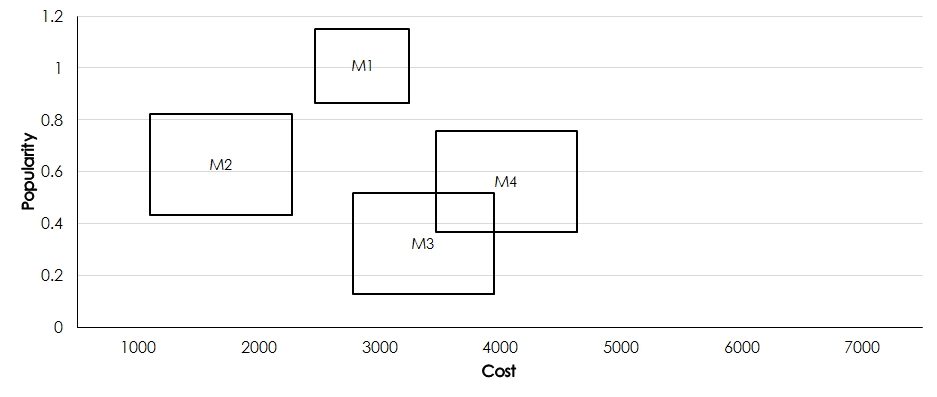
\includegraphics[width=8cm]{mbr}
\caption{Domination Relation Between Sites}
\label{fig:mbr}
\end{figure}



\section{Algorithm}
\label{algorithm}
\subsection{Preliminaries}
\label{preliminaries}
Given a dataset D on a data space defined by a set of d dimensions \{\(d_1, ..., d_d\)\}, a point p \(\in\) D is represented as p=\{\(p_1, ..., p_d\)\} where \(p_i\) is the value on dimension \(d_i\). Without loss of generality, we assume that \(\forall d_i\) : \(p_i\geq\)  0, and that smaller values are preferable.
The data set at any site Si is denoted by the MBR \(m_i(l_i,u_i)\) consisting of boundary of its data point.
We define the relations between the datasets of two different sites as:
\begin{enumerate}
\item	Site \(S_i\)  is said to fully dominate site \(S_j\) if \(u_i<l_j\).
\item	Site \(S_i\) is said to partially dominate the site \(S_j\) if \(u_i>u_j\).
\item If none of the above two cases occurs then sites are said            to be incomparable.
\end{enumerate}

In the figure \ref{fig:mbr}, \(m_2\) fully dominate \(m_1\) and hence no point in \(m_1\) can be in the k-dominant skyline and hence \(m_1\) could be pruned off from the computation. \(m_3\) partially dominates \(m_4\) hence the points which lies strictly above the upper bound (\(u_3\)) of \(m_3\) can be pruned off. Thus in general it would be beneficial to first compute the skylines in \(m_3\) then in \(m_4\). Hence , we make \(m_3\) as child of \(m_4\)  during the tree construction. The above mentioned relation between the different server sites forms the basis for our algorithm. Besides that we use one scan algorithm to find out the skylines at particular site’s data which is not pruned.

\subsection{Basic approach}
\label{basicapproach}
The basic steps involved in the algorithm are:
\begin{enumerate}
\item Collect the summarized   information (i.e. MBR) of data of each server to the originator.
\item The originator the based on  the relation between different     server defines the parent         child relation i.e. basically     creates a tree like structure     so as to execute in parallel.
\item Now , these parent child          relations will be pushed to       each server site.
\item	After this tree formation         phase , all the leaf nodes        will start computing the          k-dominant skyline in its own     database and will push the        results into the parent.
\item	The parent node or server will     compute its’ own k-dominant       set and merge it with the         result obtained from its’         children.
\item This process will keep on         going till all are results        have been accumulated to the      originator.
\end{enumerate}
\begin{algorithm}
	\caption{K-DomSkyAlgo}
	\label{alg:kdomskyalgo}
	\begin{algorithmic}[1]
		\Require Database $D$, Query $Q$
		\Ensure K-Dominant dataset k-dom
		\State for all sites do $m[i] \gets Request_MBR();$
		\State $T[]\gets Tree_Formation(sitedetails,m[i] );$
		\State Push each tree \(\in\) T to its root site
		\State k-dom= k-domskyfinder( )
		\State \Return $k-dominant dataset$
	\end{algorithmic}
\end{algorithm}
In step 1 of the algorithm ~\ref{alg:kdomskyalgo}, we use Request\_MBR() function to compute the MBR’s of each site and return to the originator. The originator server then forms the tree based on the dominance relation between different MBR. As mentioned earlier, some MBR may get fully pruned in this process. Then we forward the tree to respective to root node further find the k-dom skyline amongst node within that tree.
\\
In algorithm ~\ref{alg:Tree_Formation}, We are forming the tree based on the dominance area. If any site Si is completely dominated by any other site \(S_j\) then the site Si will be completely removed from our query computation else we find a site \(S_k\) which maximizes the partially dominance area under the site \(S_i\) and we will make \(S_i\) as parent of \(S_k\). because if we have the k-dominant and full skylines of \(S_k\) then that can prune some of the points in the \(S_i\). Continuing this way we will get our tree.
 Example in figure \ref{fig:mbr}, We can see that \(M_1\) is completely dominated by \(m_2\). So \(m_1\) will be taken out of the computations. \(m_2\) and \(m_3\) are incomparable and hence can execute in parallel.\(m_3\) partially dominates \(m_4\), hence can made \(m_4\) the child of \(m_3\).

\begin{algorithm}
	\caption{Tree\_Formation}
	\label{alg:Tree_Formation}
	\begin{algorithmic}[1]
		\Require MBR $m[i]$, $sitedetails$
		\Ensure forest $F$
		\State For all sites \(S_i\)
		\State For all sites \(S_j\)
		\State If \(S_j\) completely dominates \(S_i\) then remove \(S_i\) from the list.
		\State Else
		\State Find \(S_j\) which maximizes the dominance area of \(S_j\) under Si
		\State Assign that \(S_j\) to be parent of \(S_i\).
		\end{algorithmic}
\end{algorithm}

\begin{algorithm}
	\caption{k-domskyfinder}
	\label{alg:kdomskyfinder}
	\begin{algorithmic}[1]
		\Require Query $Q$, Forest $F={ T1,T2…..}$,filter 
		\Ensure$k-dom$,$nonk-domfullsky$
		\State If  $F$ is empty
		\State $(local_kdom,local_non-k-domfullsky)$\(\gets\)localoneScan(filter)
		\State $Else Localnonk-domfullsky= localoneScan (filter);$
		\State $remoteFilter$ =localMBR.getUpperBound( );
		\State For each tree T in forest F 
		\State (T.kdom , T.nonk-domfullsky) =k-domskyfinder(Q, T.getSubtrees,remoteFilter);
		\State Probablek-dom= Probablek-dom U T.kdom U localK-dom;
		\State Probablek-dom= Probablenonk-domfullsky U T.nonk-domfullsky U localnonk-domfullsky;
		\State $K-dom,fullsky\gets oneScanForNonLeaf( )$
	    \State \Return $k-dom,fullsky$
	\end{algorithmic}
\end{algorithm}

In algorithm ~\ref{alg:kdomskyfinder},we start from the parent nodes and goes till we encounter the leaf node, compute the k-dominant skylines and the full skylines in their local proximity. Now, this result will be returned to the parent. The parent node will compute its k-dominant skylines and the full skylines along with merging the results from its children. This process will continue till we reach the root or the originator of the query.
 \\
 In algorithm \ref{alg:oneScanForNonLeaf}, \cite{Chan:2006:FKS:1142473.1142530} In this case also we are applying the conventional one scan algorithm but with a slight modification. We here are initializing the T set to contain the probale non-k-dominant full skylines from the child sites and input will be probable k-dominants collected from descendents in tree, so as to avoid the separate merging of the results from the child sites into the parent site.
 \\
In algorithm \ref{alg:localoneScan},\cite{Chan:2006:FKS:1142473.1142530} Here we are just executing the conventional one scan algorithm for finding the k-dominant skylines and full skylines in the leaf nodes or sites in the tree.

\begin{algorithm}
	\caption{ oneScanForNonLeaf}
	\label{alg:oneScanForNonLeaf}
	\begin{algorithmic}[1]
		\Require $inputdata$,$T$
		\Ensure Result set $k-dom$, $full-sky$
		\comment {all k-dom and full-skyline of the child nodes so as to merge them into the result }
		\State run conventional onescan algo for k-dom
		\State return k-dom, full-sky.
	\end{algorithmic}
\end{algorithm}

\begin{algorithm}
	\caption{localoneScan}
	\label{alg:localoneScan}
	\begin{algorithmic}[1]
		\Require Database $D$, Query $Q$
		\Ensure Result set $A$
		\State initialize T=\(\Phi\) and R=\(\Phi\) and inputdata=localdataset
		\State run conventional onescan algo for k-dom
		\State \Return $k-dom$,$full-sky$
	\end{algorithmic}
\end{algorithm}
\section{Evaluation and Results}
\label{evaluationandresults}
\subsection{Implementation}
We are proposing the solution to the k-dominant skylines in the distributed environment. We have given our implementation in java. We are using multi-threaded TCP connection to set up communication in the distributed environment.
For parallel execution, we are using the multi-threading service of java. We evaluated the resuls by creating multiple processes on a different machine where each of these processes behaves as individual server. We distribute the data among these processes and then perform the steps as mentioned in the algorithmic section.
\subsection{Comparison among approaches}
We implemented the following three approaches for evaluation purpose. 
\begin{enumerate}
\item proposed system
\item linear chain system
\item naïve system
\end{enumerate}
Based on the result produced from the three approaches for similar distributed environment setup and diffrent input data set type, we mapped the results as follows

\begin{figure}[htp]
\centering
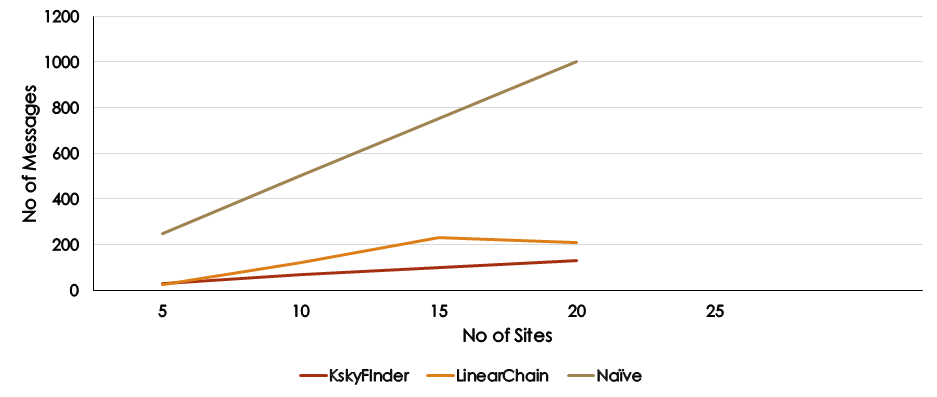
\includegraphics[width=8cm]{cor}
\caption{Result for correlated data}
\label{fig:cor}
\end{figure}
\begin{figure}[htp]
\centering
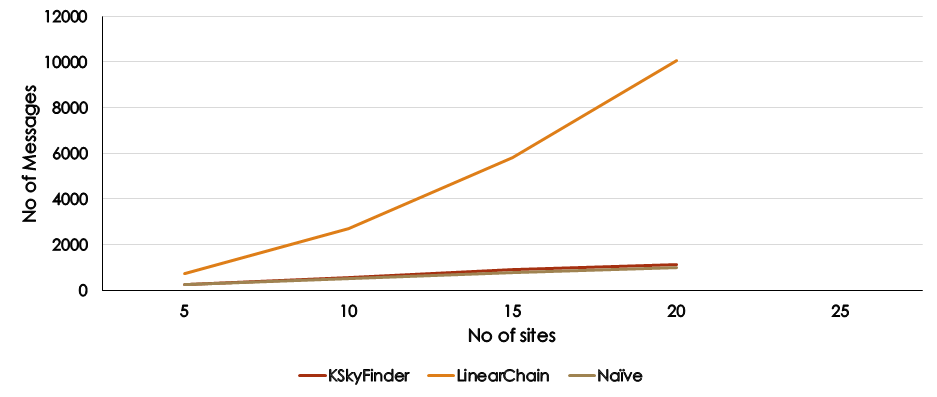
\includegraphics[width=8cm]{ant}
\caption{Result for anti-correlated data}
\label{fig:ant}
\end{figure}
\begin{figure}[htp]
\centering
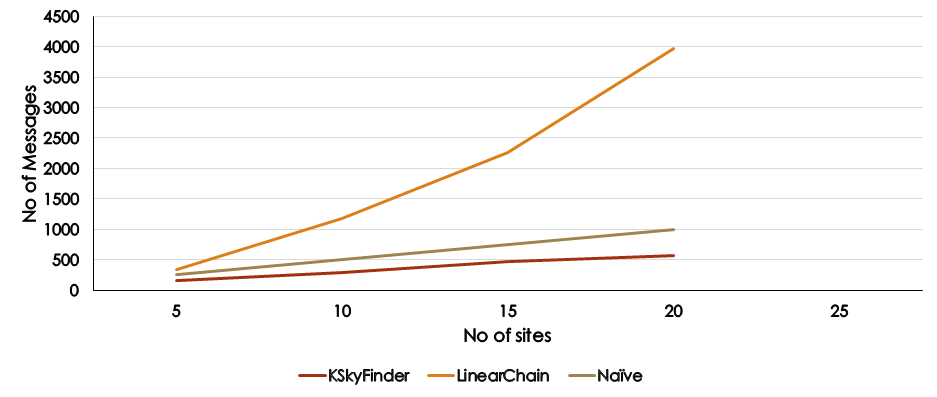
\includegraphics[width=8cm]{ind}
\caption{Result for independent data}
\label{fig:ind}
\end{figure}

\subsection{Analysis}
In case of the naive system (i.e. naive way of solving the problem), the message count observe to  be constant as its clear theoretically as well that the message count will be given by:
\\
Message count=total database size - originator database size.
\\
The time for the computation of the k-dominant skyline is less than all the other approaches as it just sends all the data to the originator server and the time taken will depend upon the bandwidth of the network used. But for large database its infeasible to occupy entire data set in memory. And may need additional overhead of temporary storage at local database of query originator.
In case of linear chain, without any ordering among sites, the number of messages over the network is very large as compared to our proposed algorithm but show less than that of the naïve system only in case of correlated data. Here the message has increased because some of the data point in the leaf node can actually be the k-dominant skyline and will traverse the whole linear chain again and again by hoping from parent node to parent of parent node until it reaches the originator the query.
Here the time taken is comparable to our algorithm. 
Proposed system: our system have significant drop against the other two approaches in case of the number of messages. But pre-processing have a drawback of increased execution time. The execution time for our system is comparable to the linear chain but much more than that of naïve system

As you go on analysing result shown in above diagram, its pretty clear that our approach gives optimum network traffic with quite noticeable difference over other approaches. Just for anti-correlated data the result is somewhat similar as we have to carry large no. of non-k-dominated full skylines as well.

\section{Conclusion}
The skyline operator is quiet useful in multi-criteria decision making applications till the number of dimensions are less. As the number of dimensions increases, we loose the insight of interesting points.Hence k-dominant skylines are more important if the number of dimensions are more. By this project, we propose an algorithm to find k-dominant skyline in distributed setting.From our analysis, we can conclude that the proposed algorithm outperforms both the naïve and the linear approaches in most of the cases when considered the network traffic.

\bibliography{K_dom}
\bibliographystyle{plain}
\end{document}

